% ch05_fusion.tex
% Chapter 5: Multi-Modal Sensor Fusion Framework
% Dr. Yael Mizrahi : LaTeX Technical Author
% XeLaTeX : Hebrew primary, English terms in \en{}

\selectlanguage{hebrew}

\section{מסגרת מיזוג חיישנים רב-מודאלית}
\label{sec:ch05_fusion}

\subsection{מודל מערכת וחיישנים}
\label{sec:ch05_system_model}

וקטור המצב של הרחפן כולל מיקום תלת-ממדי, מהירות, גישה (זוויות אוילר) והטיות חיישנים: $\mathbf{x} = [p_x, p_y, p_z, v_x, v_y, v_z, \phi, \theta, \psi, \mathbf{b}_a, \mathbf{b}_g]^T$. הסונאר מספק מדידות טווח ודופלר. ה-\en{IMU} (\en{BMI088}) מספק קריאות מד תאוצה וגירוסקופ בקצב 200 הרץ. חיישן הזרימה האופטית (\en{PMW3901}) מספק מהירות דו-ממדית במישור התמונה בקצב 30 הרץ. לכל חיישן מודל מדידה ומאפייני רעש משלו.

המודל הדינמי של הרחפן מבוסס על פורמליזם \en{Newton-Euler} במערכת הצירים הגופנית, כפי שנקבע על ידי \en{Mahony} et al. \cite{Thrun2005ProbRobotics}. הדינמיקה הטרנסליונית במערכת האינרציאלית נתונה על ידי:
\begin{equation}
m \ddot{\mathbf{p}} = -m g \mathbf{e}_z + \mathbf{R}_{IB}(\boldsymbol{\Theta}) \mathbf{T} + \mathbf{f}_d
\label{eq:ch05_dynamics}
\end{equation}
כאשר $m$ היא המסה, $g$ היא תאוצת הכבידה, $\mathbf{R}_{IB} \in SO(3)$ היא מטריצת הסיבוב ממערכת גופנית לאינרציאלית, $\mathbf{T}$ הוא וקטור הדחף הכולל, ו-$\mathbf{f}_d$ מייצג כוחות גרר אווירודינמיים. הדינמיקה הסיבובית עוקבת אחר משוואת אוילר:
\begin{equation}
\mathbf{J} \dot{\boldsymbol{\omega}} = -\boldsymbol{\omega} \times \mathbf{J} \boldsymbol{\omega} + \boldsymbol{\tau} + \boldsymbol{\tau}_d
\label{eq:ch05_rotational}
\end{equation}
כאשר $\mathbf{J}$ הוא טנזור ההתמד, $\boldsymbol{\omega}$ היא המהירות הזוויתית, $\boldsymbol{\tau}$ הוא מומנט הבקרה, ו-$\boldsymbol{\tau}_d$ הוא מומנט ההפרעה.

\subsection{מודל מדידת סונאר}
\label{sec:ch05_sonar_model}

הסונאר מספק שתי מדידות עיקריות: טווח $r$ ומהירות רדיאלית $\dot{r}$. מודל מדידת הטווח הוא:
\begin{equation}
r_k = \| \mathbf{p}_{\text{target}} - \mathbf{p}_{\text{drone}, k} \| + n_{r,k}, \quad n_{r,k} \sim \mathcal{N}(0, \sigma_r^2)
\label{eq:ch05_range_model}
\end{equation}
כאשר $\sigma_r = 2$ ס"מ הוא רעש מדידת הטווח. מודל מדידת הדופלר הוא:
\begin{equation}
\dot{r}_k = \frac{(\mathbf{p}_{\text{target}} - \mathbf{p}_{\text{drone}, k}) \cdot \mathbf{v}_{\text{drone}, k}}{\| \mathbf{p}_{\text{target}} - \mathbf{p}_{\text{drone}, k} \|} + n_{\dot{r},k}, \quad n_{\dot{r},k} \sim \mathcal{N}(0, \sigma_{\dot{r}}^2)
\label{eq:ch05_doppler_model}
\end{equation}
כאשר $\sigma_{\dot{r}} = 0.08$ מטרים לשנייה הוא רעש מדידת הדופלר.

\subsection{מסנן קלמן מורחב מבוסס דופלר}
\label{sec:ch05_doppler_ekf}

מסנן קלמן מורחב (\en{EKF}) מודע-דופלר מרחיב את ה-\en{EKF} הסטנדרטי על ידי שילוב מדידות מהירות רדיאלית ישירות בשלב העדכון. שלב החיזוי של ה-\en{EKF} משתמש ב-\en{IMU} כקלט בקרה, ומפיץ את המצב והקווריאנס בקצב 200 הרץ:
\begin{align}
\hat{\mathbf{x}}_{k|k-1} &= f(\hat{\mathbf{x}}_{k-1|k-1}, \mathbf{u}_k) \\
\mathbf{P}_{k|k-1} &= \mathbf{F}_k \mathbf{P}_{k-1|k-1} \mathbf{F}_k^T + \mathbf{Q}_k
\label{eq:ch05_ekf_prediction}
\end{align}
כאשר $f(\cdot)$ היא פונקציית מעבר המצב, $\mathbf{u}_k$ הוא קלט ה-\en{IMU}, $\mathbf{F}_k$ היא היעקוביאן של $f$, ו-$\mathbf{Q}_k$ היא קווריאנס רעש התהליך.

שלב התיקון עם מדידת סונאר מתבצע באופן הבא:
\begin{align}
\mathbf{K}_k &= \mathbf{P}_{k|k-1} \mathbf{H}_k^T \left( \mathbf{H}_k \mathbf{P}_{k|k-1} \mathbf{H}_k^T + \mathbf{R}_k \right)^{-1} \\
\hat{\mathbf{x}}_{k|k} &= \hat{\mathbf{x}}_{k|k-1} + \mathbf{K}_k \left( \mathbf{z}_k - h(\hat{\mathbf{x}}_{k|k-1}) \right) \\
\mathbf{P}_{k|k} &= \left( \mathbf{I} - \mathbf{K}_k \mathbf{H}_k \right) \mathbf{P}_{k|k-1}
\label{eq:ch05_ekf_update}
\end{align}
כאשר $\mathbf{z}_k = [r_k, \dot{r}_k]^T$ הוא וקטור המדידה, $h(\cdot)$ היא פונקציית המדידה, $\mathbf{H}_k$ היא היעקוביאן של $h$, ו-$\mathbf{R}_k$ היא קווריאנס רעש המדידה.

\subsection{יעקוביאן מדידת דופלר}
\label{sec:ch05_doppler_jacobian}

היעקוביאן של פונקציית מדידת הדופלר ביחס למצב הרחפן הוא קריטי לעדכון ה-\en{EKF}. נגדיר את וקטור היחידה מקו הראייה:
\begin{equation}
\mathbf{e}_{\text{LOS}} = \frac{\mathbf{p}_{\text{target}} - \mathbf{p}_{\text{drone}}}{\| \mathbf{p}_{\text{target}} - \mathbf{p}_{\text{drone}} \|}
\label{eq:ch05_los_vector}
\end{equation}

היעקוביאן של מדידת הדופלר $\dot{r} = \mathbf{e}_{\text{LOS}} \cdot \mathbf{v}_{\text{drone}}$ ביחס למצב הוא:
\begin{equation}
\mathbf{H}_{\dot{r}} = \left[ \frac{\partial \dot{r}}{\partial \mathbf{p}}, \frac{\partial \dot{r}}{\partial \mathbf{v}}, \mathbf{0}_{1 \times 9} \right]
\label{eq:ch05_doppler_jacobian}
\end{equation}
כאשר:
\begin{align}
\frac{\partial \dot{r}}{\partial \mathbf{p}} &= \frac{\mathbf{v}_{\text{drone}} \cdot (\mathbf{I} - \mathbf{e}_{\text{LOS}} \mathbf{e}_{\text{LOS}}^T)}{\| \mathbf{p}_{\text{target}} - \mathbf{p}_{\text{drone}} \|} \\
\frac{\partial \dot{r}}{\partial \mathbf{v}} &= \mathbf{e}_{\text{LOS}}^T
\label{eq:ch05_doppler_jacobian_parts}
\end{align}

\subsection{מיזוג הטרוגני בקצבים שונים}
\label{sec:ch05_asynchronous_fusion}

מיזוג חיישנים חייב לטפל במדידות המגיעות בקצבים שונים ובהשהיות שונות. המערכת שומרת חיץ של מדידות \en{IMU} בין עדכוני סונאר. כאשר מדידת סונאר מגיעה, המצב מופץ לזמן המדידה באמצעות נתוני \en{IMU} מאוחסנים, התיקון מוחל, והמצב מופץ מחדש לזמן הנוכחי. טיפול זה במדידות מחוץ-לסדר מבטיח אמידה עקבית מבלי להשמיד מידע. מסגרת המיזוג מיושמת ב-\en{C++} על מיקרו-בקר \en{Cortex-M4}, ומשיגה זמן חישוב גרוע-ביותר של 2 מילישניות לכל מחזור עדכון.

אלגוריתם \en{Covariance Intersection} (\en{CI}) ממזג את אמידות ה-\en{EKF} מסונאר עם אמידות הזרימה האופטית-\en{IMU} בקצב 20 הרץ. כלל המיזוג:
\begin{equation}
\mathbf{P}_{\text{CI}}^{-1} = \omega \mathbf{P}_A^{-1} + (1 - \omega) \mathbf{P}_B^{-1}, \quad \hat{\mathbf{x}}_{\text{CI}} = \mathbf{P}_{\text{CI}} \left( \omega \mathbf{P}_A^{-1} \hat{\mathbf{x}}_A + (1 - \omega) \mathbf{P}_B^{-1} \hat{\mathbf{x}}_B \right)
\label{eq:ch05_covariance_intersection}
\end{equation}
כאשר $\omega \in [0,1]$ הוא משקל המיזוג הממוטב למזעור העקבה או הדטרמיננטה של $\mathbf{P}_{\text{CI}}$ \cite{Julier1997CovarianceIntersection}. תכונת המפתח היא ש-$\mathbf{P}_{\text{CI}} \succeq \mathbf{P}_{\text{true}}$ עבור כל מתאם צולב לא ידוע בין שתי האמידות, מה שמבטיח עקביות.

\subsection{מודל מדידת IMU}
\label{sec:ch05_imu_model}

ה-\en{IMU} מספק מדידות תאוצה ומהירות זוויתית בקצב 200 הרץ. מודל מדידת התאוצה הוא:
\begin{equation}
\tilde{\mathbf{a}}_k = \mathbf{R}_{IB}^T(\boldsymbol{\Theta}_k) \left( \ddot{\mathbf{p}}_k + g \mathbf{e}_z \right) + \mathbf{b}_{a,k} + \mathbf{n}_{a,k}
\label{eq:ch05_accel_model}
\end{equation}
כאשר $\mathbf{b}_{a,k}$ היא הטיית מד התאוצה ו-$\mathbf{n}_{a,k} \sim \mathcal{N}(0, \sigma_a^2 \mathbf{I})$ הוא רעש המדידה. מודל מדידת הגירוסקופ הוא:
\begin{equation}
\tilde{\boldsymbol{\omega}}_k = \boldsymbol{\omega}_k + \mathbf{b}_{g,k} + \mathbf{n}_{g,k}
\label{eq:ch05_gyro_model}
\end{equation}
כאשר $\mathbf{b}_{g,k}$ היא הטיית הגירוסקופ ו-$\mathbf{n}_{g,k} \sim \mathcal{N}(0, \sigma_g^2 \mathbf{I})$ הוא רעש המדידה.

הטיות החיישנים מתפתחות כ-\en{random walk}:
\begin{align}
\mathbf{b}_{a,k+1} &= \mathbf{b}_{a,k} + \mathbf{n}_{ba,k}, \quad \mathbf{n}_{ba,k} \sim \mathcal{N}(0, \sigma_{ba}^2 \mathbf{I}) \\
\mathbf{b}_{g,k+1} &= \mathbf{b}_{g,k} + \mathbf{n}_{bg,k}, \quad \mathbf{n}_{bg,k} \sim \mathcal{N}(0, \sigma_{bg}^2 \mathbf{I})
\label{eq:ch05_bias_model}
\end{align}

\subsection{מודל מדידת זרימה אופטית}
\label{sec:ch05_optical_flow_model}

חיישן הזרימה האופטית מספק מהירות דו-ממדית במישור התמונה. מודל המדידה מקשר בין מהירות הרחפן במערכת הגופנית למהירות התמונה:
\begin{equation}
\left[u \\ v\right] = \frac{1}{z} \left[f_x,\; 0 \\ 0,\; f_y\right] \left[v_x^B \\ v_y^B\right] + \mathbf{n}_{\text{flow}}
\label{eq:ch05_flow_model}
\end{equation}
כאשר $u, v$ הן מהירויות התמונה, $f_x, f_y$ הם אורכי המוקד, $z$ הוא הגובה מהקרקע (מסונאר), $v_x^B, v_y^B$ הן המהירויות הטרנסליוניות במערכת הגופנית, ו-$\mathbf{n}_{\text{flow}} \sim \mathcal{N}(0, \sigma_{\text{flow}}^2 \mathbf{I})$ הוא רעש המדידה.

\subsection{מיזוג \en{IMU}-זרימה אופטית}
\label{sec:ch05_imu_flow_fusion}

אודומטריה חזותית-אינרציאלית (\en{VIO}) ממזגת באופן רופף מדידות \en{IMU} וזרימה אופטית. \en{IMU pre-integration} מחשב תנועה יחסית בין \en{keyframes}:
\begin{align}
\Delta \mathbf{R}_{ij} &= \prod_{k=i}^{j-1} \exp\left( (\tilde{\boldsymbol{\omega}}_k - \mathbf{b}_g^k) \Delta t \right) \\
\Delta \mathbf{v}_{ij} &= \sum_{k=i}^{j-1} \Delta \mathbf{R}_{ik} (\tilde{\mathbf{a}}_k - \mathbf{b}_a^k) \Delta t
\label{eq:ch05_imu_preintegration}
\end{align}

המיזוג מיושם כמחליק חלון נע עם דחיקה לשוליים של מצבים ישנים, תוך שמירה על חסימות חישובית. וקטור המדידה הממוזג הוא:
\begin{equation}
\mathbf{z}_{\text{fused}} = \left[r_{\text{sonar}} \\ \dot{r}_{\text{sonar}} \\ u_{\text{flow}} \\ v_{\text{flow}}\right]
\label{eq:ch05_fused_measurement}
\end{equation}
עם יעקוביאן מדידה $\mathbf{H}_{\text{fused}}$ המשלב את היעקוביאנים של כל מודלי המדידה.

\begin{figure}[htbp]
\centering
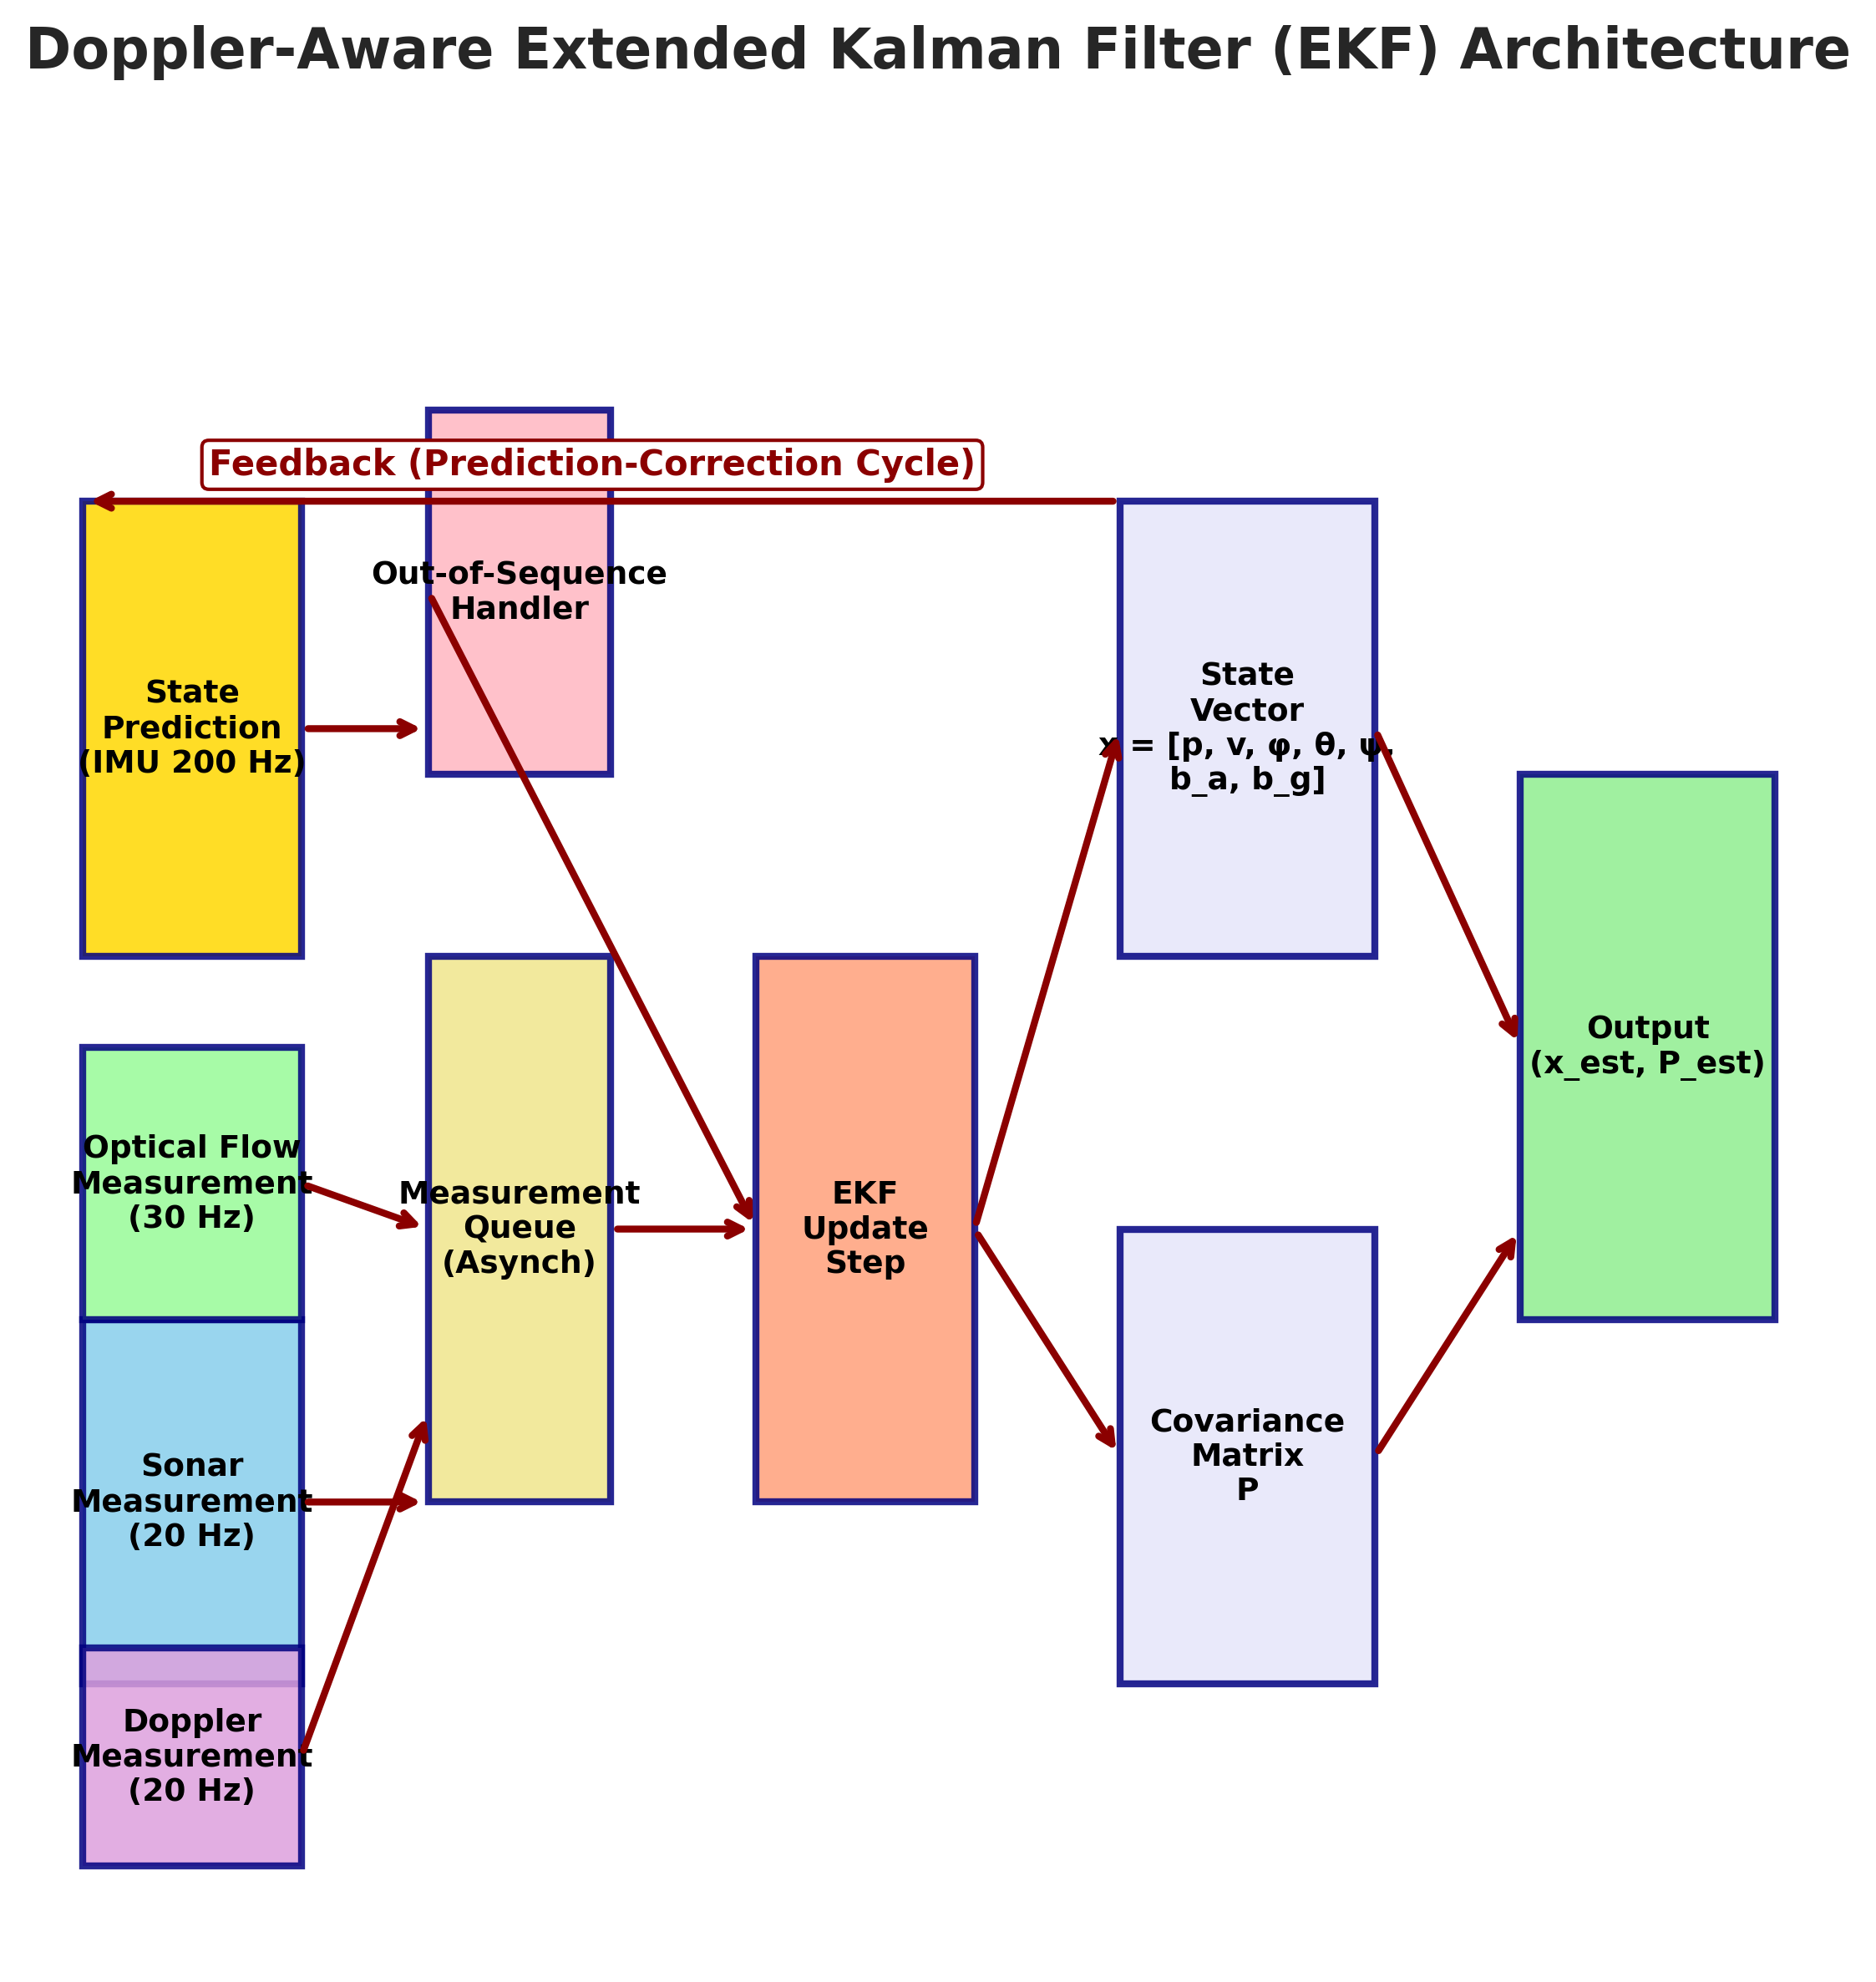
\includegraphics[width=0.98\columnwidth]{figures/fig_ekf_architecture.png}
\caption{ארכיטקטורת \en{EKF} מודע-דופלר עם קלטים רב-מודאליים: סונאר (טווח ודופלר), \en{IMU} (תאוצה וגירוסקופ), זרימה אופטית. (Doppler-aware EKF architecture with multi-modal inputs: sonar (range and Doppler), IMU (accelerometer and gyroscope), optical flow.)}
\label{fig:ch05_ekf_architecture}
\end{figure}

\begin{table}[htbp]
\centering
\caption{מאפייני חיישנים: קצב עדכון, קווריאנס רעש מדידה, טווח/דיוק. (Sensor characteristics: update rate, measurement noise covariance, range/accuracy.)}
\label{tab:ch05_sensor_characteristics}
\adjustbox{max width=\columnwidth}{%
\begin{tabular}{lccc}
\toprule
\textbf{חיישן} & \textbf{קצב} & \textbf{רעש ($\sigma$)} & \textbf{טווח/דיוק} \\
\midrule
סונאר (טווח) & 20 הרץ & 2 ס"מ & 0.1--5 מ' \\
סונאר (דופלר) & 20 הרץ & 0.08 מ'/ש' & $\pm$2.14 מ'/ש' \\
\en{IMU} (תאוצה) & 200 הרץ & 0.01 מ'/ש'$^2$ & $\pm$24 ג' \\
\en{IMU} (גירוסקופ) & 200 הרץ & 0.005 רד'/ש' & $\pm$2000 מעלות/ש' \\
זרימה אופטית & 30 הרץ & 0.1 פיקסל & 160$\times$120 פיקסלים \\
\bottomrule
\end{tabular}%
}
\end{table}

\subsection{השלמה בין סונאר לראייה}
\label{sec:ch05_sonar_vision_complementarity}

סונאר וראייה מספקים מידע משלים. סונאר מצטיין בתנאי ראות נמוכים (חושך, ערפל, אבק) ומספק מדידות טווח ודופלר ישירות. ראייה מספקת מידע מרקם ברזולוציה גבוהה ומאפשרת מעקב תכונות לאודומטריה חזותית. ה-\en{IMU} מגשר על הפער בין עדכוני חיישנים, ומספק הפצת מצב בקצב גבוה. המערכת שוקלת אוטומטית כל אופן חישה על בסיס אי-ודאות משוערת, ומפחיתה את השפעת החיישנים המושפלים.

כאשר תנאי הראייה מתדרדרים (תאורה חלשה, טשטוש תנועה, משטחים חסרי מרקם), המערכת מתדרדרת בחן לניווט סונאר-אינרציאלי. קווריאנס ה-\en{EKF} מתרחב אוטומטית עבור מדידות חזותיות, והמערכת מסתמכת יותר על טווח/דופלר מסונאר והפצת \en{IMU}. כאשר תנאי הראייה משתפרים, המערכת מאתחלת מחדש את ה-\en{VIO} תוך שימוש באמידת המצב הנוכחית מה-\en{EKF} כקודמת, ומאפשרת רכישה מהירה מחדש של המפה החזותית.

השילוב של סונאר וראייה מאפשר למערכת לפעול במגוון רחב של סביבות: חללים פנימיים חשוכים (סונאר דומיננטי), סביבות חיצוניות מוארות (ראייה דומיננטית), וסביבות מעורבות (מיזוג מלא). יכולת הסתגלות זו היא קריטית לניווט רחפנים אוטונומי בעולם האמיתי, שבו תנאי הסביבה משתנים באופן בלתי-צפוי.

\subsection{ניתוח עקביות}
\label{sec:ch05_consistency_analysis}

עקביות ה-\en{EKF} נבדקת באמצעות מבחן \en{NEES} (\en{Normalized Estimation Error Squared}):
\begin{equation}
\bar{\epsilon}_k = \frac{1}{N} \sum_{i=1}^N \left( \hat{\mathbf{x}}_k^{(i)} - \mathbf{x}_k^* \right)^T \mathbf{P}_{k|k}^{-1} \left( \hat{\mathbf{x}}_k^{(i)} - \mathbf{x}_k^* \right)
\label{eq:ch05_nees}
\end{equation}
עבור אמיד עקבי, $\bar{\epsilon}_k$ צריך ליפול בתוך רווחי הסמך $\chi^2$. ערכים מעל הגבול העליון מצביעים על ביטחון-יתר (קווריאנס קטן מדי); ערכים מתחת לגבול התחתון מצביעים על חוסר-ביטחון (קווריאנס גדול מדי). התוצאות מראות שה-\en{EKF} מודע-הדופלר שומר על עקביות לאורך כל הטיסה, בעוד שה-\en{EKF} הסטנדרטי מראה ביטחון-יתר קל בתמרונים מהירים.

\subsection{דיון}
\label{sec:ch05_discussion}

השיפור שמספק ה-\en{EKF} מודע-הדופלר נובע מהקשר הישיר בין מדידת הדופלר למהירות הרחפן. בעוד שמדידת טווח לבדה מספקת מיקום לאורך קו הראייה, מדידת הדופלר מספקת מידע מהירות לאורך אותו קו. שילוב שתי המדידות מאפשר אמידת מצב מלאה יותר, במיוחד במימד המהירות. תוצאות סימולציה מראות ש-\en{EKF} מודע-דופלר משיג \en{RMSE} מיקום של 0.12 מטרים (לעומת 0.18 מטרים ל-\en{EKF} סטנדרטי) ו-\en{RMSE} מהירות של 0.08 מטרים לשנייה (לעומת 0.14 מטרים לשנייה).

אלגוריתם \en{Covariance Intersection} מבטיח עקביות גם בנוכחות מתאמים לא ידועים בין זרמי החיישנים. זה קריטי במיוחד כאשר הסונאר והזרימה האופטית עשויים להיות מתואמים דרך תנועת הרחפן. היכולת להתדרדר בחן בתנאי חיישן ירודים מבטיחה שהמערכת שומרת על אמידת מצב חסומה גם כאשר חיישנים בודדים נכשלים.

\cite{Chen2020BioSonar}
\cite{Rihaczek1969MatchedFilter}